%! TEX root = main.tex
\begin{filecontents}{conservedvector.tex}

\centering
\begin{figure}
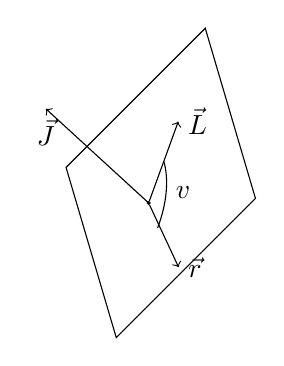
\begin{tikzpicture}[rotate around z=45, rotate around x=-45]
\draw (0,-0.3,0) -- (2.5,-0.3,0) -- (2.5,2.5,0) -- (0,2.5,0) -- cycle;
\draw[->] (1.,1.,0)node[draw,circle,inner sep=0] (o) {} -- (1.5,1.5,2)node[below] {$\vec{J}$};
\draw[->] (o) -- ++(295:0.9cm)node[right] {$\vec{r}$};
\draw[->] (o) -- ++(70:1.1cm)node[right] {$\vec{L}$}node [midway] (aux){};
\draw (aux) arc (0:-50:1) node[midway,right] {$v$};
\end{tikzpicture}

\label{fig:Lenztikz}

\end{figure}

\end{filecontents}

\begin{filecontents}{cylsang.tex}
    %\begin{tikzpicture}[tdplot_main_coords]
%%    \draw[-latex] (0,0,0) -- (1,0,0) node[pos=1.1]{$x$};
%%    \draw[-latex] (0,0,0) -- (0,1,0) node[pos=1.1]{$y$};
%%    \draw[-latex] (0,0,0) -- (0,0,1) node[pos=1.1]{$z$};
%  \begin{scope}[canvas is xy plane at z=0]
%   \path (0,0) coordinate[label=below:$O$] (O);
%   \draw[dashed] (\tdplotmainphi:\myr) arc(\tdplotmainphi:\tdplotmainphi+180:\myr);
%   \draw[dashed] (\angA:\myr) coordinate (A) -- (\angB:\myr) coordinate (B)
%    node[pos=-0.1] {$A$} node[pos=1.1] {$B$};
%   \draw[thick] (\tdplotmainphi:\myr) coordinate(BR) arc(\tdplotmainphi:\tdplotmainphi-180:\myr)
%   coordinate(BL);
%  \end{scope} 
\begin{axis}[
axis lines=center,
axis on top,
every inner z axis line/.append style={opacity=0},
xlabel={$x$}, ylabel={$y$}, zlabel={$t$},
domain=0:1,
y domain=0:2*pi,
xmin=-1.5, xmax=1.5,
ymin=-1.5, ymax=1.5, zmin=0.0,zmax=1.2,ztick={1},
every axis x label/.style={at={(rel axis cs:0,0.5,0)},anchor=south},
every axis y label/.style={at={(rel axis cs:0.5,0,0)},anchor=north},
every axis z label/.style={at={(rel axis cs:0.5,0.5,0.9)},anchor=west},
samples=30]
\addplot3 [surf, colormap/blackwhite, shader=flat] ({x*cos(deg(y))},{x*sin(deg(y))},{x});
\addplot3 [domain=0:360,samples y=1,name path=top,draw=none] ({1*cos(deg(x))},{1*sin(deg(x))},{1});
\path[name path=zline] (0,0,0) -- (0,0,1.2) coordinate(ztop);
\path[name intersections={of=top and zline,by={aux1}}];
\draw[-latex] (aux1) -- (ztop);
%standard tikz coordinate definition using x, y, z coords
\coordinate (O) at (0,0,0);

%tikz-3dplot coordinate definition using x, y, z coords
%\pgfmathsetmacro{\axone}{0.5}
%\pgfmathsetmacro{\ayone}{0.3}
%\pgfmathsetmacro{\azone}{0.4}
%\pgfmathsetmacro{\axtwo}{0.3}
%\pgfmathsetmacro{\aytwo}{0.5}
%\pgfmathsetmacro{\aztwo}{0}
%\coordinate (P1) at (\axone,\ayone,\azone);
%\coordinate (P2) at (\axtwo,\aytwo,\aztwo);
%\coordinate (P3) at (\axone+\axtwo,\ayone+\aytwo,\azone+\aztwo);
%\fill[red,opacity=0.2] (O) -- (P1) -- (P3) -- (P2) -- cycle;
%\draw[vector] (O) -- (P1);
%\draw[vector] (O) -- (P2);
\addplot3[
    samples y=0,
    smooth, thick, color=blue,
    domain=0:sqrt(2)
    ] ({0},{4-2*x^2},{x}) coordinate [pos=0.3] (trihedron origin) ;
\draw [-latex,color=violet,thick] (trihedron origin) -- +(axis direction cs:0,0,1)
    node [anchor=west] {$ds$};
\end{axis}
\end{filecontents}
